\documentclass[12pt,a4paper]{article}

\usepackage[margin=1in]{geometry}
\usepackage{amsmath, amssymb, amsthm}
\usepackage{mathtools}
\usepackage{enumitem}
\usepackage{booktabs}
\usepackage{array}
\usepackage{xcolor}
\usepackage{tikz}
\usetikzlibrary{arrows.meta, positioning}

\setlength{\parindent}{0pt}
\setlength{\parskip}{6pt}

\newtheoremstyle{lecturestyle}
  {8pt}
  {8pt}
  {\normalfont}
  {}
  {\bfseries}
  {.}
  {0.5em}
  {}

\theoremstyle{lecturestyle}
\newtheorem{definition}{Definition}
\newtheorem{example}{Example}
\newtheorem{proposition}{Proposition}
\newtheorem{corollary}{Corollary}
\newtheorem{remark}{Remark}

\newenvironment{answer}
{\par\textbf{Answer.}\ }
{\hfill$\square$\par}

\newcommand{\Prob}{\mathbb{P}}
\newcommand{\E}{\mathbb{E}}
\newcommand{\Var}{\operatorname{Var}}

\title{\textbf{Lecture 10: Random Walks and Branching Processes}}
\author{MA4034: Time Series and Stochastic Processes}
\date{}

\begin{document}
\maketitle

\section{Discrete Random Walks}

A random walk is a Markov chain that moves step by step through a state space. In a one-dimensional discrete random walk, the states are usually integers:
\[
S=\{\ldots,-2,-1,0,1,2,\ldots\}.
\]

At each time step, the chain moves to a neighbouring state:
\[
i\to i+1
\quad\text{or}\quad
i\to i-1.
\]

Let
\[
\Prob(i\to i+1)=p,
\qquad
\Prob(i\to i-1)=1-p=q.
\]
Then
\[
p+q=1.
\]

\begin{center}
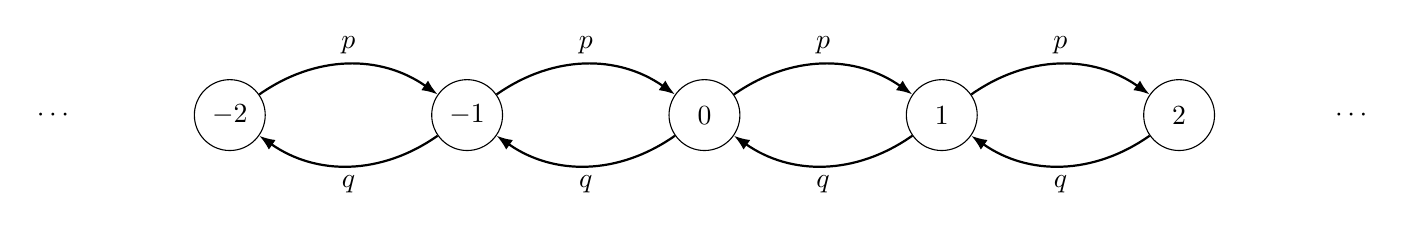
\begin{tikzpicture}[
  state/.style={circle, draw, minimum size=9mm},
  edge/.style={-{Latex[length=2mm]}, thick},
  bend angle=35
]
\node (leftdots) {$\cdots$};
\node[state, right=14mm of leftdots] (m2) {$-2$};
\node[state, right=21mm of m2] (m1) {$-1$};
\node[state, right=21mm of m1] (z) {$0$};
\node[state, right=21mm of z] (p1) {$1$};
\node[state, right=21mm of p1] (p2) {$2$};
\node[right=14mm of p2] (rightdots) {$\cdots$};

\draw[edge] (m2) edge[bend left] node[above] {$p$} (m1);
\draw[edge] (m1) edge[bend left] node[below] {$q$} (m2);
\draw[edge] (m1) edge[bend left] node[above] {$p$} (z);
\draw[edge] (z) edge[bend left] node[below] {$q$} (m1);
\draw[edge] (z) edge[bend left] node[above] {$p$} (p1);
\draw[edge] (p1) edge[bend left] node[below] {$q$} (z);
\draw[edge] (p1) edge[bend left] node[above] {$p$} (p2);
\draw[edge] (p2) edge[bend left] node[below] {$q$} (p1);
\end{tikzpicture}
\end{center}

\textbf{Analogy.} Imagine standing on a number line. At every second, you flip a biased coin. If it is heads, you move one step to the right. If it is tails, you move one step to the left. Your position after many flips is a random walk.

\section{Returning to the Same State}

In a one-dimensional random walk, the chain cannot return to the same state in an odd number of steps.

For example, starting at state $0$:
\[
0\to 1
\]
after one step, or
\[
0\to -1.
\]
So after one step, it cannot be back at $0$.

To return to the starting state, the number of right moves must equal the number of left moves. Therefore the total number of steps must be even.

Thus,
\[
p_{ii}^{(2n-1)}=0,
\qquad n=1,2,\ldots
\]

\subsection{Even-Step Return Probability}

To return to state $i$ after $2n$ steps, the random walk must take:
\[
n\text{ steps to the right}
\]
and
\[
n\text{ steps to the left}.
\]

The number of possible orders is
\[
\binom{2n}{n}.
\]

Each such path has probability
\[
p^nq^n=(pq)^n.
\]

Therefore,
\[
p_{ii}^{(2n)}
=
\binom{2n}{n}p^nq^n
=
\frac{(2n)!}{n!n!}\{p(1-p)\}^n.
\]

\section{Using Stirling's Formula}

For large $n$, Stirling's formula says
\[
n!\sim n^n e^{-n}\sqrt{2\pi n}.
\]

Using Stirling's formula, we obtain
\[
p_{ii}^{(2n)}
\sim
\frac{(4p(1-p))^n}{\sqrt{\pi n}}.
\]

This approximation helps us decide whether the state is recurrent or transient.

\section{Recurrence and Transience of the One-Dimensional Random Walk}

Recall the recurrence criterion:
\[
\text{state }i\text{ is recurrent}
\quad\Longleftrightarrow\quad
\sum_{n=1}^{\infty}p_{ii}^{(n)}=\infty.
\]

\subsection{Case 1: Fair Random Walk, $p=\frac12$}

If
\[
p=\frac12,
\]
then
\[
4p(1-p)=4\left(\frac12\right)\left(\frac12\right)=1.
\]

Therefore,
\[
p_{ii}^{(2n)}
\sim
\frac{1}{\sqrt{\pi n}}.
\]

So
\[
\sum_{n=1}^{\infty}p_{ii}^{(2n)}
\sim
\sum_{n=1}^{\infty}\frac{1}{\sqrt{\pi n}}.
\]

The series
\[
\sum_{n=1}^{\infty}\frac1{\sqrt{n}}
\]
diverges. Therefore the fair one-dimensional random walk is recurrent.

However, the expected return time is infinite, so it is \textbf{null recurrent}.

\[
\boxed{p=\frac12 \quad\Longrightarrow\quad \text{null recurrent}.}
\]

\subsection{Case 2: Biased Random Walk, $p\neq \frac12$}

If
\[
p\neq \frac12,
\]
then
\[
4p(1-p)<1.
\]

Let
\[
r=4p(1-p).
\]
Then
\[
0<r<1.
\]

So
\[
p_{ii}^{(2n)}
\sim
\frac{r^n}{\sqrt{\pi n}}.
\]

Since $r^n$ decreases geometrically, the series
\[
\sum_{n=1}^{\infty}\frac{r^n}{\sqrt{\pi n}}
\]
converges.

Therefore,
\[
\sum_{n=1}^{\infty}p_{ii}^{(n)}<\infty.
\]

Hence the biased one-dimensional random walk is transient.

\[
\boxed{p\neq\frac12 \quad\Longrightarrow\quad \text{transient}.}
\]

\subsection{Stationary Distribution}

The one-dimensional random walk on
\[
\mathbb{Z}=\{\ldots,-2,-1,0,1,2,\ldots\}
\]
has no stationary distribution.

Reason:
\begin{itemize}[leftmargin=1.2cm]
    \item If $p=\frac12$, the chain is null recurrent, not positive recurrent.
    \item If $p\neq\frac12$, the chain is transient.
\end{itemize}

For an irreducible Markov chain, a stationary distribution exists only when the chain is positive recurrent. Therefore, in either case, there is no stationary distribution.

\[
\boxed{\text{No stationary distribution for the one-dimensional random walk on }\mathbb{Z}.}
\]

\section{Multi-Dimensional Random Walks}

A multi-dimensional random walk needs two or more variables to describe its state.

For example, in two dimensions:
\[
S_n=(X_n,Y_n).
\]

Here the state space is
\[
\mathbb{Z}^2=\{(x,y):x,y\in\mathbb{Z}\}.
\]

\textbf{Analogy.} In one dimension, you walk on a number line. In two dimensions, you walk on a grid. In three dimensions, you move around in space.

\subsection{Two-Dimensional Random Walk}

For a simple symmetric two-dimensional random walk, the chain moves randomly on the integer grid. A key result is:
\[
\Prob(S_{2n}=(0,0)\mid S_0=(0,0))
\sim
\frac{1}{\pi n}.
\]

Therefore,
\[
\sum_{n=1}^{\infty}\Prob(S_{2n}=(0,0)\mid S_0=(0,0))
\sim
\sum_{n=1}^{\infty}\frac1{\pi n}.
\]

The harmonic series diverges:
\[
\sum_{n=1}^{\infty}\frac1n=\infty.
\]

So the two-dimensional simple symmetric random walk is recurrent.

Since the expected return time is infinite, it is null recurrent.

\[
\boxed{\text{Two-dimensional simple symmetric random walk is null recurrent}.}
\]

\subsection{Three or More Dimensions}

In dimensions
\[
d\geq 3,
\]
the simple symmetric random walk is transient.

Intuitively, in high dimensions there are many more directions and many more states to visit. The walk has a good chance of drifting away and never returning to the original state.

\begin{corollary}
The symmetric simple random walk in dimension $d$ is recurrent for
\[
d=1,2
\]
and transient for
\[
d\geq 3.
\]
\end{corollary}

\section{Branching Processes}

A branching process is a stochastic process used to model population growth and extinction.

Let
\[
Z_n=\text{number of individuals in generation }n.
\]

Usually,
\[
Z_0=1,
\]
meaning the population starts with one individual.

Each individual independently produces a random number of children. The number of children produced by one individual is called the \textbf{offspring distribution}.

\begin{center}
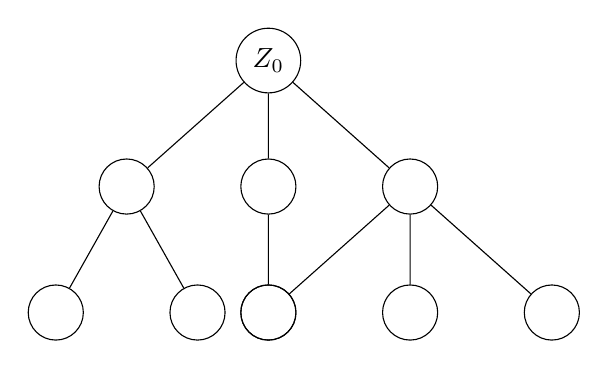
\begin{tikzpicture}[
  person/.style={circle, draw, minimum size=7mm},
  edge/.style={-{Latex[length=2mm]}, thick},
  level distance=16mm,
  sibling distance=18mm
]
\node[person] {$Z_0$}
  child {node[person] {}
    child {node[person] {}}
    child {node[person] {}}
  }
  child {node[person] {}
    child {node[person] {}}
  }
  child {node[person] {}
    child {node[person] {}}
    child {node[person] {}}
    child {node[person] {}}
  };
\end{tikzpicture}
\end{center}

\textbf{Analogy.} Think of a family tree. One person has some children. Each child then has their own children. The branching process counts how many people are in each generation.

\subsection{Recursive Definition}

Let
\[
X_k=\text{number of children produced by the }k\text{th individual}.
\]

If there are $Z_{n-1}$ individuals in generation $n-1$, then the number of individuals in generation $n$ is
\[
Z_n=\sum_{k=1}^{Z_{n-1}}X_k,
\qquad n=1,2,\ldots
\]

Here:
\begin{itemize}[leftmargin=1.2cm]
    \item $k$ is the index of the individual in generation $n-1$,
    \item $X_k$ is the number of children produced by that individual,
    \item $Z_n$ is the total number of children produced by all individuals in generation $n-1$.
\end{itemize}

Through $Z_n$, we can study:
\begin{itemize}[leftmargin=1.2cm]
    \item population extinction,
    \item population growth.
\end{itemize}

\section{Probability Generating Functions}

\begin{definition}[Probability Generating Function]
If $X$ is a non-negative integer-valued random variable, its probability generating function is
\[
G(s)=\E[s^X].
\]
\end{definition}

If
\[
\Prob(X=k)=p_k,
\]
then
\[
G(s)=\sum_{k=0}^{\infty}p_ks^k.
\]

\textbf{Analogy.} A probability generating function stores the whole offspring distribution inside one function. The coefficient of $s^k$ tells us the probability of having $k$ children.

\section{Population Extinction}

Let
\[
E=\{\text{event that the population eventually becomes extinct}\}.
\]

Extinction means that for some generation $n$,
\[
Z_n=0.
\]

Once
\[
Z_n=0,
\]
there are no individuals left to reproduce, so the process remains at zero forever.

\subsection{PGF Recursion}

Let the offspring distribution have pgf $G(s)$. Let the pgf of $Z_n$ be $G_n(s)$.

Then
\[
G_1(s)=G(s)
\]
and
\[
G_n(s)=G_{n-1}(G(s)),
\qquad n=2,3,\ldots
\]

The extinction probability is
\[
\Prob(E)=\lim_{n\to\infty}\Prob(Z_n=0)
=
\lim_{n\to\infty}G_n(0).
\]

\begin{proposition}[Extinction Probability]
Consider a branching process where the offspring distribution has pgf $G$. Let $E$ be the event of extinction. Then
\[
\Prob(E)
\]
is the smallest solution in $[0,1]$ to
\[
s=G(s).
\]
\end{proposition}

Note that
\[
s=1
\]
is always a solution of
\[
s=G(s),
\]
because
\[
G(1)=1.
\]

But the extinction probability is the \textbf{smallest} solution in $[0,1]$.

\section{Worked Extinction Example}

\begin{example}
Consider a population of cells. Each cell either dies or reproduces according to
\[
X=
\begin{cases}
0, & \text{with probability } \frac14,\\
2, & \text{with probability } \frac34.
\end{cases}
\]
Find the probability of extinction.
\end{example}

\begin{answer}
The offspring pgf is
\[
G(s)=\E[s^X].
\]

Since $X=0$ with probability $1/4$ and $X=2$ with probability $3/4$,
\[
G(s)=\frac14s^0+\frac34s^2.
\]
So
\[
G(s)=\frac14+\frac34s^2.
\]

The extinction probability is the smallest solution in $[0,1]$ to
\[
s=G(s).
\]

Thus,
\[
s=\frac14+\frac34s^2.
\]

Multiply by 4:
\[
4s=1+3s^2.
\]

Rearrange:
\[
3s^2-4s+1=0.
\]

Factor:
\[
(3s-1)(s-1)=0.
\]

Therefore,
\[
s=\frac13
\quad\text{or}\quad
s=1.
\]

The extinction probability is the smallest solution in $[0,1]$:
\[
\boxed{\Prob(E)=\frac13.}
\]
\end{answer}

\section{Population Growth}

Let
\[
\mu=\E[X]
\]
be the mean number of children per individual, and let
\[
\sigma^2=\Var(X)
\]
be the variance of the offspring distribution.

\begin{proposition}[Mean and Variance of $Z_n$]
For a branching process with $Z_0=1$,
\[
\E[Z_n]=\mu^n.
\]
Also,
\[
\Var(Z_n)=
\begin{cases}
n\sigma^2, & \mu=1,\\[4pt]
\displaystyle
\sigma^2\mu^{n-1}\frac{\mu^n-1}{\mu-1}, & \mu\neq 1.
\end{cases}
\]
\end{proposition}

\subsection{Interpretation of $\mu$}

The value
\[
\mu=\E[X]
\]
is the average number of children produced by one individual.

\[
\begin{array}{c|c|c}
\text{Condition} & \text{Extinction Probability} & \text{Interpretation}\\
\hline
\mu\leq 1 & \Prob(E)=1 & \text{population becomes extinct eventually}\\
\mu>1 & \Prob(E)<1 & \text{population may survive}
\end{array}
\]

If
\[
\mu<1,
\]
then each individual produces less than one child on average, so the population tends to die out.

If
\[
\mu=1,
\]
the process is critical. Extinction still occurs with probability 1, but it may take a long time.

If
\[
\mu>1,
\]
the process is supercritical. There is a positive probability that the population survives forever.

\section{Worked Growth Example}

\begin{example}
For the cell example,
\[
X=
\begin{cases}
0, & \text{with probability } \frac14,\\
2, & \text{with probability } \frac34,
\end{cases}
\]
find $\mu$, $\E[Z_n]$, and explain whether extinction is certain.
\end{example}

\begin{answer}
The mean offspring number is
\[
\mu=\E[X].
\]

Therefore,
\[
\mu=0\left(\frac14\right)+2\left(\frac34\right).
\]

So
\[
\mu=\frac32.
\]

Since
\[
\mu>1,
\]
the process is supercritical. Therefore extinction is not certain:
\[
\Prob(E)<1.
\]

From the previous example, the extinction probability is
\[
\Prob(E)=\frac13.
\]

The expected population size in generation $n$ is
\[
\E[Z_n]=\mu^n.
\]

Thus,
\[
\boxed{\E[Z_n]=\left(\frac32\right)^n.}
\]
\end{answer}

\section{Worked Examples}

\begin{example}[Return Probability of a Random Walk]
In a one-dimensional random walk, suppose $p=0.4$ and $q=0.6$. Find the probability that the chain returns to its starting state after 4 steps.
\end{example}

\begin{answer}
Returning after 4 steps means that the chain must take 2 right steps and 2 left steps.

Thus,
\[
p_{ii}^{(4)}
=
\binom{4}{2}p^2q^2.
\]

Substitute
\[
p=0.4,
\qquad
q=0.6.
\]

Then
\[
p_{ii}^{(4)}
=
6(0.4)^2(0.6)^2.
\]

So
\[
p_{ii}^{(4)}
=
6(0.16)(0.36)
=
0.3456.
\]
\end{answer}

\begin{example}[Classifying a One-Dimensional Random Walk]
Classify the one-dimensional random walk with $p=0.5$.
\end{example}

\begin{answer}
Since
\[
p=\frac12,
\]
the one-dimensional random walk is fair.

The fair one-dimensional random walk is recurrent, but the expected return time is infinite.

Therefore it is null recurrent.

\[
\boxed{\text{Null recurrent}.}
\]
\end{answer}

\begin{example}[Extinction Probability]
Suppose the offspring distribution is
\[
\Prob(X=0)=\frac12,
\qquad
\Prob(X=2)=\frac12.
\]
Find the extinction probability.
\end{example}

\begin{answer}
The pgf is
\[
G(s)=\frac12+\frac12s^2.
\]

The extinction probability is the smallest solution in $[0,1]$ to
\[
s=G(s).
\]

Thus,
\[
s=\frac12+\frac12s^2.
\]

Multiply by 2:
\[
2s=1+s^2.
\]

Rearrange:
\[
s^2-2s+1=0.
\]

Factor:
\[
(s-1)^2=0.
\]

Thus the only solution is
\[
s=1.
\]

Therefore,
\[
\boxed{\Prob(E)=1.}
\]

The mean number of children is
\[
\mu=0\left(\frac12\right)+2\left(\frac12\right)=1.
\]
This is the critical case, so extinction occurs with probability 1.
\end{answer}

\section{Summary}

\begin{itemize}[leftmargin=1.2cm]
    \item A one-dimensional random walk moves from $i$ to $i+1$ with probability $p$ and to $i-1$ with probability $1-p$.
    \item A one-dimensional random walk can return to the same state only after an even number of steps.
    \item The even-step return probability is
    \[
    p_{ii}^{(2n)}=\binom{2n}{n}p^n(1-p)^n.
    \]
    \item By Stirling's formula,
    \[
    p_{ii}^{(2n)}\sim \frac{(4p(1-p))^n}{\sqrt{\pi n}}.
    \]
    \item If $p=1/2$, the one-dimensional random walk is null recurrent.
    \item If $p\neq1/2$, the one-dimensional random walk is transient.
    \item Simple symmetric random walks are recurrent in dimensions 1 and 2, and transient in dimensions 3 or more.
    \item A branching process models population growth generation by generation.
    \item The population size satisfies
    \[
    Z_n=\sum_{k=1}^{Z_{n-1}}X_k.
    \]
    \item The extinction probability is the smallest solution in $[0,1]$ to
    \[
    s=G(s).
    \]
    \item If $\mu\leq1$, extinction occurs with probability 1.
    \item If $\mu>1$, extinction occurs with probability less than 1.
\end{itemize}

\section{Essay-Type Questions}

\begin{enumerate}[label=\textbf{Q\arabic*.}, leftmargin=1.2cm]
    \item Define a one-dimensional random walk and draw its transition diagram. Explain why it cannot return to the same state in an odd number of steps.
    \item Derive the formula
    \[
    p_{ii}^{(2n)}=\binom{2n}{n}p^n(1-p)^n.
    \]
    \item Explain how Stirling's formula is used to classify the one-dimensional random walk as recurrent or transient.
    \item State the recurrence result for simple symmetric random walks in dimensions 1, 2, and 3 or more.
    \item Define a branching process and explain the meaning of $Z_n$ and $X_k$.
    \item Explain how probability generating functions are used to find extinction probabilities.
    \item For an offspring distribution with pgf $G(s)$, explain why the extinction probability is the smallest solution of $s=G(s)$.
    \item Suppose $\Prob(X=0)=1/4$ and $\Prob(X=2)=3/4$. Find the extinction probability and expected population size at generation $n$.
\end{enumerate}

\section{Answers to Essay-Type Questions}

\subsection*{Answer 1}

A one-dimensional random walk is a Markov chain on
\[
S=\{\ldots,-2,-1,0,1,2,\ldots\}
\]
where the chain moves from state $i$ to $i+1$ with probability $p$ and from state $i$ to $i-1$ with probability $1-p$.

It cannot return to the same state in an odd number of steps because returning requires the number of right moves to equal the number of left moves. Therefore the total number of moves must be even.

\subsection*{Answer 2}

To return to state $i$ after $2n$ steps, the random walk must take exactly $n$ right steps and $n$ left steps.

The number of possible arrangements of these steps is
\[
\binom{2n}{n}.
\]
Each arrangement has probability
\[
p^n(1-p)^n.
\]
Therefore,
\[
p_{ii}^{(2n)}=\binom{2n}{n}p^n(1-p)^n.
\]

\subsection*{Answer 3}

Stirling's formula gives
\[
n!\sim n^ne^{-n}\sqrt{2\pi n}.
\]
Using it,
\[
p_{ii}^{(2n)}
\sim
\frac{(4p(1-p))^n}{\sqrt{\pi n}}.
\]

If $p=1/2$, then $4p(1-p)=1$, so
\[
p_{ii}^{(2n)}\sim \frac1{\sqrt{\pi n}}.
\]
The series of these terms diverges, so the chain is recurrent. Since the expected return time is infinite, it is null recurrent.

If $p\neq1/2$, then $4p(1-p)<1$. The return probabilities decrease geometrically, so the sum converges. Therefore the chain is transient.

\subsection*{Answer 4}

For the simple symmetric random walk:
\[
d=1 \quad \Rightarrow \quad \text{recurrent},
\]
\[
d=2 \quad \Rightarrow \quad \text{recurrent},
\]
and
\[
d\geq3 \quad \Rightarrow \quad \text{transient}.
\]

In dimensions 1 and 2, the walk returns to the starting point with probability 1. In dimensions 3 or more, there is a positive probability that the walk never returns.

\subsection*{Answer 5}

A branching process models population size over generations. Let
\[
Z_n=\text{number of individuals in generation }n.
\]
Usually,
\[
Z_0=1.
\]

Let
\[
X_k=\text{number of children produced by the }k\text{th individual}.
\]
If generation $n-1$ has $Z_{n-1}$ individuals, then generation $n$ has
\[
Z_n=\sum_{k=1}^{Z_{n-1}}X_k
\]
individuals.

\subsection*{Answer 6}

The probability generating function of the offspring distribution is
\[
G(s)=\E[s^X].
\]
If $G_n(s)$ is the pgf of $Z_n$, then
\[
G_n(s)=G_{n-1}(G(s)).
\]

The extinction probability is
\[
\Prob(E)=\lim_{n\to\infty}\Prob(Z_n=0).
\]
Since
\[
\Prob(Z_n=0)=G_n(0),
\]
we get
\[
\Prob(E)=\lim_{n\to\infty}G_n(0).
\]

\subsection*{Answer 7}

Let
\[
s=\Prob(E)
\]
be the extinction probability. If the first individual has $k$ children, then extinction occurs only if all $k$ descendant lines become extinct.

Since each line becomes extinct with probability $s$, the probability that all $k$ lines become extinct is
\[
s^k.
\]
Averaging over all possible values of $k$ gives
\[
s=G(s).
\]

The extinction probability is the smallest solution in $[0,1]$ because $s=1$ is always a solution, but in supercritical cases there may be a smaller solution representing the actual extinction probability.

\subsection*{Answer 8}

The offspring pgf is
\[
G(s)=\frac14+\frac34s^2.
\]

The extinction probability satisfies
\[
s=G(s).
\]
Thus,
\[
s=\frac14+\frac34s^2.
\]
Multiplying by 4:
\[
4s=1+3s^2.
\]
So
\[
3s^2-4s+1=0.
\]
Factoring:
\[
(3s-1)(s-1)=0.
\]
Thus
\[
s=\frac13
\quad\text{or}\quad
s=1.
\]
The smallest solution in $[0,1]$ is
\[
\Prob(E)=\frac13.
\]

The mean offspring number is
\[
\mu=0\left(\frac14\right)+2\left(\frac34\right)=\frac32.
\]
Therefore,
\[
\E[Z_n]=\mu^n=\left(\frac32\right)^n.
\]

\end{document}
